\documentclass[sigplan,screen]{acmart}
\settopmatter{printacmref=false}
\renewcommand\footnotetextcopyrightpermission[1]{}
\usepackage{amsmath}
\usepackage{listings}
\usepackage{color}
\usepackage{tabularx}
\usepackage{multirow}
\usepackage{float}
\usepackage{graphics}
\definecolor{dkgreen}{rgb}{0,0.6,0}
\definecolor{gray}{rgb}{0.5,0.5,0.5}
\definecolor{mauve}{rgb}{0.58,0,0.82}

\lstset{frame=tb,
  language=Java,
  aboveskip=3mm,
  belowskip=3mm,
  showstringspaces=false,
  columns=flexible,
  basicstyle={\small\ttfamily},
  numbers=none,
  numberstyle=\tiny\color{gray},
  keywordstyle=\color{blue},
  commentstyle=\color{dkgreen},
  stringstyle=\color{mauve},
  breaklines=true,
  breakatwhitespace=true,
  tabsize=3
}
\begin{document}

\title{Building Bug Pattern Detection Tool using Java Parser}
\subtitle{\url{https://github.com/Aruna-Pala/javaparser-bug-detector}}
\author{Aruna Devi Pala}
\email{arunadevi.pala@mail.concordia.ca}
\affiliation{%
  \institution{Concordia University}
  \city{Montreal}
  \state{Quebec}
  \country{Canada}
}


\begin{abstract}
  
  Static bug detection tools are becoming popular and developers around the world are integrating these tools with their code to find bugs,improve the readability and to ensure correctness and completeness of code before deploying it to the server \cite{ernst2003static}.Bugs present in the code can be developed statistically or Dynamically. Using Static analysis developers can find bugs faster than dynamic analysis \cite{truong2004static}.Static bug detection analysis done without running the Java Code which is possible using integrated development platform such as Eclipse but Dynamic analysis is done during run time.
  
  In this paper we have implemented bug patterns to detect bugs in the code base followed by detecting developed bug patterns on one of the large-scale system which is CloudStack by cloning code from \url{https://github.com/apache/cloudstack/tree/4.9}. I have used JavaParser \cite{hosseini2013javaparser} open source library that can parse Java files into abstract syntax trees.

\end{abstract}
\keywords{JavaParser, Bug Pattern, Maven, JUnit,Java}
\maketitle
\pagestyle{plain}

\section{Introduction}
Bugs are prevalent in many software development systems.
There are many existing static bug detection techniques which industries have adopted for tracking bugs in their software \cite{nam2019bug}. For an average industry code the number of bugs per 1,000 lines of code has been estimated to range between 0.5 and 25 \cite{mcconnell2006software} Software contains unnoticed bugs even after several years of deployment. Reliability of software is one crucial Quality that we have to ensure before implementing any techniques. Several approaches are used to ensure the code Quality which includes bug detection implementation using both static and dynamic analysis,
testing the software in phases as unit testing, integration testing, system testing and so on.

To improve the reliability of software I have implemented static analysis tools to detect bug patterns in java classes. For analyzing code, have studied about two analysis tools which are Eclipse JDT and Java Parser. After analysis I thought of implementing bug patterns using Java Parser because it is easy to use and configuration can be done in few lines whereas Eclipse JDT comes with lot of dependencies,OSGi and an extremely complex configuration.This Paper covers three bug patterns that consists of the following:\\
(1) \textbf{\emph{Class defines hashCode() but not equals()}:} if a class overrides the \emph{hashcode} method but not \emph{equals} method causing a function that consists \emph{equals} method to fail.\\
(2) \textbf{\emph{equals() method does not check for null argument}:} if an \emph{equals} method overrides in a class and the \emph{equal} method is passed with
\emph{NULL Argument} then the \emph{equal} method returns Null pointer exception which does not check for null value.\\
(3) \textbf{\emph{Inadequate logging information in catch blocks}:} duplicate logging statements in dfferent catch blocks of the same try block may cause debugging difficulties and can be confusing
for the developer while debugging code.

To ensure detection of bugs in code I have used Junit framework to create test cases for all three bug patterns mentioned.Using Junit we can write test cases while developing the software,Since our bug pattern is build on top of Maven I have chosen to use Junit as test framework because it supports Maven and Ant projects.  Also have done detection analysis of implemented bug patterns on CloudStack 4.9.

\section{Detection Approach}
I have used JavaParser library to analyze and detect bug patterns in the software system developed.JavaParser is an open Source library used to parse Java Code.
\subsection{Bug Pattern Architecture}
I have followed the Maven standard layout \cite{smart2005introduction} to implement the bug patterns.Initially Created \emph{javaparser-bug-detector} Maven project in eclipse version 4.21. All the dependencies of the project are managed in pom.xml where the JavaParser library and its version 3.6.12 are handled. At the root of the solution, there is a filesToParse folder that contains java parser files and source folder \emph{src} which contains \emph{main} and \emph{test} directories.test directory contains all the JUnit test Cases to analyze the bug patterns. Main source directory consists of:\\
-\textbf{\emph{main.java}}: This is an entry point to start the execution of the program.\\
-\textbf{\emph{CommonUtil.java}:} contains common utility functions to handle file I/O operations such as  getLineNumber, getFunctionName, getMethodDeclaration, deleteReport and generateReport.\\
-\textbf{\emph{DirExplorer.java}:} to handle exploration of folders recursively.\\
-\textbf{\emph{Interfaces directory}:} which consists IBug and IChecker interfaces.\\
-\textbf{\emph{BugPattern}:} Contains three bug patterns that are \emph{Class defines hashCode() but not equals()}, \emph{equals() method does not check for null argument} and \emph{Inadequate logging information in catch blocks}.\\
-\textbf{\emph{Checker}:} This is the common functions for all three bug patterns which is explained further in program Listing 1 as shown below:\\

\begin{lstlisting}[caption={Common Checker function for all the three bug Patterns},captionpos=b]
public List<BugPattern> check(File projectDir) {
 List<BugPattern> bugPatterns = new ArrayList<>();
  new DirExplorer((level, path, file) ->     path.endsWith(".java"), (level, path, file) -> {
   try {
    // Declare the variables for Bug Patterns provided
   new VoidVisitorAdapter<Object>() {
    @Override
    public void visit(MethodDeclaration md, Object arg)
    {
     super.visit(md, arg);
   /** Here is the specific code for Bug  Patterns mentioned
   * class defines hashcode() but not equals, 
   * equals() method does not check for null argument 
   * Inadequate logging information in catch blocks When the conditions are met
   **/
        if (bug conditions are met) {
           // Get the line number
            int lineNo = Util.getlineNo(n);
            // Get the method name
            String functionName = Util.getFunctionName(n);
            // Add the bug pattern to the list
            bugPatterns.add(newBugPatternName(lineNo, file,
            functionName));
                       }
                   }
               }.visit(JavaParser.parse(file), null);

           } catch (IOException e) {
               new RuntimeException(e);
           }
       }).explore(projectDir);
       return bugPatterns;
}
\end{lstlisting}

\subsection{Report Generation}

Once all the three implemented checkers are executed and all three bug patterns are found and a \emph{txt} file is generated with filename as bugpattern.txt  under report folder.To generate reports, inside \emph{CommonUtil.java} a \emph{generatereport} method will be called that create files and write the bug patterns found.Checkers for all three bug patterns is explained further as :\\
(1) \textbf{\emph{Class defines hashCode() but not equals()}} is a visitor object that inspects each method of the software or any provided file.For each of the methods found our tool will try to identify the return type and name of the method.If this name is \emph{hashcode} and return type is string with no arguments and if such method is found then boolean value is set to true specifying that hashcode method is found.It also checks whether the given class overrides \emph{equals} method then it will set bug pattern to false.\\
(2) \textbf{\emph{equals() method does not check for null argument}} uses a visitor object that inspects \emph{equals()} method in the provided file.In the program \emph{equals} method is compared to an object with \emph{null}. This comparison will always return false since the object is not null,if the object is null program will throw NullPointerException. This bug pattern is handled by overriding \emph{equals} method which checks object is null and returns false.\\
(3) \textbf{\emph{Inadequate logging information in catch blocks}} uses a visitor that inspects logging statements in try catch exceptions.The error messages are stored in ArrayList object.If there exists \emph{duplicate} error messages then tool will notify the user about the error message found.\\

Below Listing 2 explains how the report is generated in \emph{.txt} form:

\begin{lstlisting}[caption={Generate reports using bugpatterns},captionpos=b]
\\bugpattern.txt
public static void generateReport(List<BugPattern> bugPatternsList) {
try {
	boolean filecreated = createFiles();
	if (filecreated) {
	FileWriter myWriter = new FileWriter(reportFilePath);
	for (BugPattern bugPattern : bugPatternsList) {
		System.out.println(bugPattern.toString());
		myWriter.write(bugPattern.toString());
	}
	myWriter.close();
	System.out.println("Successfully wrote to the file.");
	}
} catch (IOException e) {
	System.out.println("An error occurred.");
	e.printStackTrace();
}
\end{lstlisting}

Table 1 explains the three bug pattern summary that is implemented and tested in the program. If we run main.java then from above listing 2 function bugpattern.txt will be generated under report folder which contains the below Table 1 summary.
\begin{table}[H]
  \caption{Bug Pattern}
  \label{tab}
  \begin{tabular}{ll}
    \toprule
    BugPattern &Summary\\
    \midrule
    \toprule
    HE & fileName='HashcodeWithoutEquals.java'\\
    &functionName='hashCode', line=3\\
    \midrule
    IL & fileName='InadequateLogInfoIn\\
    &CatchBlock.java'\\ 
    &functionName='InadequateMain', line=10\\
    \midrule
    NP & fileName='EqualsWithoutNull\\
    &Argument.java'\\ 
    &functionName='equals', line=5\\
  \bottomrule
\end{tabular}
\end{table}

\section{Test Cases Designing}

Each Bug pattern has both positive and negative test scenarios in the java test folder that validates the bug pattern when it exists in Java classes and not when it does not exists. 

Listing 3 shows postive and negative unit test case scenario of \textbf{\emph{HashcodeWithoutEquals}} method.The other bug patterns can be tested in similar way which is included in the source code of Git repository mentioned in this document.
\begin{lstlisting}[caption={Test case Scenarios for all the three bug patterns TestJavaparserBugDetector.java},captionpos=b]

public class TestJavaparserBugDetector {
	@Test
	public void testEqualWithHashcode() {
        List<BugPattern> bugPatterns = new HashcodeWithoutEqualsChecker().check(new File("filesToParse/filesToParseTest/
        HashcodeWithEquals.java"));

		Assert.assertEquals(0, bugPatterns.size());
	}

	@Test
	public void testEqualWithoutHashcode() {
		List<BugPattern> bugPatterns = new HashcodeWithoutEqualsChecker().check(new File("filesToParse/HashcodeWithoutEquals.java"));

		Assert.assertEquals(1, bugPatterns.size());
		Assert.assertEquals("HashcodeWithoutEquals.java", bugPatterns.get(0).getFilename());
		Assert.assertEquals("hashCode", bugPatterns.get(0).getFunctionName());
		Assert.assertEquals(3, bugPatterns.get(0).getLine());
	}
        
	/** Here we will write all positive and negative test scenarios
    * for other bug patterns
    * testDuplicateLoggingStatementIn
    * CatchBlockOfSameTryWithAdequateInfo.java
    * testEqualsWithoutNullArgumentChecker.java
    **/
}
\end{lstlisting}
\begin{figure}[H]
    \centering
    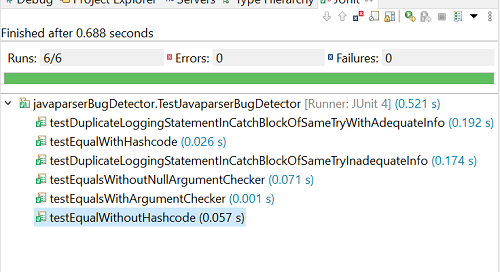
\includegraphics[width=0.7\columnwidth]{JUnit Trace.png}
    \caption{JUnitTrace from Eclipse}
    \label{fig:JunitTest}
\end{figure}

Figure 2 Shows that complete test coverage of implemented bug patterns. We can see Code coverage as 100\%
\begin{figure}[H]
    \centering
    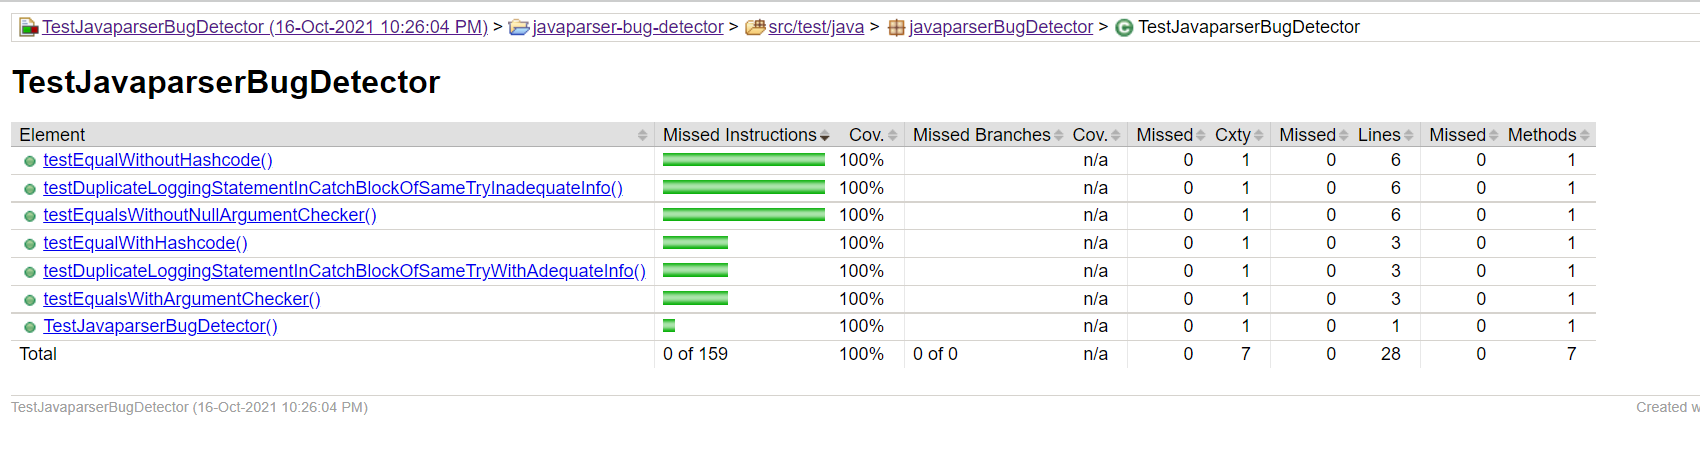
\includegraphics[width=0.7\columnwidth]{code coverage.png}
    \caption{JUnit Test Coverage results}
    \label{fig:Code Coverage}
\end{figure}
\section{Detection results and Discussion}
To validate our bug pattern implementation we ran our static bug pattern tool on CloudStack 4.9.After analysis we found total 19 instances on CloudStack System among which one Class have "HE" bug \emph{HashcodeWithoutEquals}, two classes with "IL" bugs \emph{InadequateLogInfoInCatchBlockChecker} and all remaining 16 bugs are "NP" \emph{EqualsWithoutNullArgumentChecker}. 

This Section includes how to setup the environment to run bug pattern tool on one of the large scale system "CloudStack 4.9" followed by detection results of CloudStack after validating.
\subsection{Environment Setup}
By following below steps we can do environmental setup for the project and validate bug patterns:
(1) Clone this repo: "git clone https://github.com/Aruna-Pala/javaparser-bug-detector.git"\\
(2) cd javaparser-bug-detector into the folder of the repo you just cloned\\
(3) Install maven dependencies mvn install\\
(4) Run the bugpattern app using mvn exec:java\\ -Dexec.mainClass=javaparserBugDetector.Main

\subsection{Running tool on CloudStack}

Below are the Steps to run out tool on CloudStack:\\
(1)Clone the Apache CloudStack source code using "git clone https://github.com/apache/cloudstack.git" into bug pattern project inside fileToParse folder.\\
(2) Install maven dependencies mvn install.\\
(3) Run the bugpattern app using mvn exec:java\\ -Dexec.mainClass=javaparserBugDetector.Main\\
(4) Now you can see all the three bug patterns are detected in the CloudStack repo and the report logs will be generated in bugpattern.txt.

Table 2 shows the results of our static bug analysis tool on Apache CloudStack. 

Identifier HE in the table means \textcolor{blue}{\emph{HashCodeWithoutequals}}, filename field indicates in which file hashcode bug pattern exists with class containing hashcode without equals method which is followed by line number in that particular file. 

Identifier IL in the table means \textcolor{blue}{\emph{InadequateLogInfoInCatchBlock}},in CloudStack it is detected that in same file we have 2 different try catch blocks with same logging statements.

Identifier NP means \textcolor{blue}{\emph{EqualsWithoutNullArgument}}, in CloudStack it is detected that 16 classes have equals method which does not check for null argument all the details with line number and file name is mentioned in Table 2.

\begin{table}[H]
\caption{Detection results of CloudStack}
\begin{tabular}{|l|l|l|}
\hline
\textbf{fileName}& \textbf{Identifier}& \textbf{lineNumber} \\ \hline
\begin{tabular}[c]{@{}l@{}}PhysicalNetworkVO.java\end{tabular} & HE  & 164  \\ \hline
\begin{tabular}[c]{@{}l@{}}XenServerStorageProcessor.java\end{tabular} &IL  & 648 \\ \hline
\begin{tabular}[c]{@{}l@{}}XenServerStorageProcessor.java\end{tabular} &IL  & 646 \\ \hline
\begin{tabular}[c]{@{}l@{}}BaseNiciraEntity.java\end{tabular} &NP  & 73 \\ \hline
\begin{tabular}[c]{@{}l@{}}TemplateZoneResponse.java\end{tabular} &NP  & 114 \\ \hline
\begin{tabular}[c]{@{}l@{}}VifAttachment.java\end{tabular} &NP  & 66 \\ \hline
\begin{tabular}[c]{@{}l@{}}Match.java\end{tabular} &NP  & 99 \\ \hline
\begin{tabular}[c]{@{}l@{}}SolidFireUtil.java\end{tabular} &NP  & 1014 \\ \hline
\begin{tabular}[c]{@{}l@{}}AclRule.java\end{tabular} &NP  & 194 \\ \hline
\begin{tabular}[c]{@{}l@{}}NeutronNetwork.java\end{tabular} &NP  & 115 \\ \hline
\begin{tabular}[c]{@{}l@{}}NeutronPort.java\end{tabular} &NP  & 145 \\ \hline
\begin{tabular}[c]{@{}l@{}}SecurityGroupManagerImpl.java\end{tabular} &NP  & 256 \\ \hline
\begin{tabular}[c]{@{}l@{}}ConnectedAgentAttache.java\end{tabular} &NP  & 80 \\ \hline
\begin{tabular}[c]{@{}l@{}}NeutronNetworkWrapper.java\end{tabular} &NP  & 54 \\ \hline
\begin{tabular}[c]{@{}l@{}}SecurityRule.java\end{tabular} &NP  & 119 \\ \hline
\begin{tabular}[c]{@{}l@{}}NeutronPortWrapper.java\end{tabular} &NP  & 54 \\ \hline
\begin{tabular}[c]{@{}l@{}}AgentAttache.java\end{tabular} &NP  & 334 \\ \hline
\begin{tabular}[c]{@{}l@{}}SolidFireUtil.java\end{tabular} &NP  & 678 \\ \hline
\begin{tabular}[c]{@{}l@{}}SolidFireUtil.java\end{tabular} &NP  & 867 \\ \hline
\end{tabular}
\end{table}

There was Scalability issue while running code on large system like CloudStack. We have to increase our memory and change checkers according to the size of the project. Using system with more RAM can reduce time consumption during analysis of the bug pattern tool.

\section{Conclusion and Future Work}
In this Paper, We have implemented static analysis tool to detect bugs in source code. We have implemented three different bug patterns and analysis done on large scale system which is Apache CloudStack.Have tested all the three bug patterns on dummy java files which results in three patterns with the line numbers.

In future, will develop other bug patterns and try to do analysis on other large scale systems and also will increase Scalability to improve efficiency and performance.

\bibliographystyle{ACM-Reference-Format}
\bibliography{BugPattern}
\end{document}
\endinput

